\chapter{Utility Classes}

Next to the main modules described in the previous chapter, {\tt
  libbats} offers a collection of utility classes. We will discuss
these here.

\lstset{numbers=none}

\section{Singleton}
\label{secSingleton}

Many modules of the library are so called singletons, so we will give
a short introduction about what this is and how they are used. The
singleton pattern is a design pattern that makes sure that there is no
more than one instance of a certain class. For instance, there is only
one Queen of The Netherlands, it would make no sense to create
multiple instances. In the singleton design pattern, special measures
are taken to prevent you from copying the single instance or creating
new objects of the class. This pattern is used in the library for
modules for which it makes no sense and for which it could cause
problems if there are multiple instances. This is for instance the
case for modules keeping track of states, such as the {\tt Localizer}
and the {\tt AgentModel}, and a module for maintaining the connection
with the server.

In this library, singletons are implemented by the {\tt Singleton<T>}
template class. It offers the static {\tt getInstance()} method to
request a reference to the single instance of class {\tt T}. For
instance, the following shows how to get a reference to the {\tt
  WorldModel}:
\begin{lstlisting}[frame=single]
WorldModel& wm = Singleton<WorldModel>::getInstance();
\end{lstlisting}
For each singleton class of the library, a {\tt typedef} is set for
the {\tt Singleton<T>} instantiation of that class, formed by
prefixing the class name with a capital S. So another way to write the
previous example would be:
\begin{lstlisting}[frame=single]
WorldModel& wm = SWorldModel::getInstance();
\end{lstlisting}

If you want to use the {\tt Singleton<T>} template to create
singletons of your own class, make sure it adhears to the following
points:
\begin{itemize}
\item Your class must have a default constructor.
\item Make all constructors, including the copy constructor, of your
  class private.
\item Make the assignment operator, {\tt operator=}, private.
\item Define {\tt Singleton<T>}, instantiated with your own class, as
  friend of your class.
\end{itemize}
If you do this, your class definition will look like this:
%\lstset{numbers=left,numberstyle=\small}
\begin{lstlisting}[frame=single]
class MySingleton
{
  friend class bats::Singleton<MySingleton>;
private:
  // Default constructor
  MySingleton() {}
  // Copy constructor, not implemented
  MySingleton{MySingleton const& other);
  // Assignment operator, not implemented
  MySingleton& operator=(MySingleton const& other);
public:
  // Some public stuff
};
// libbats style singleton typedef
typedef bats::Singleton<MySingleton> SMySingleton;
\end{lstlisting}

\section{Distribution}

Agents often have to work with uncertainty and probability
distributions. For instance, vision data received from the simulator
is limited and noisy, therefore location estimates derived from this
data are just that: estimates, with a certain variability. To deal
with this, {\tt libbats} offers the {\tt Distribution} template. This
template supports distributions over any number of dimensions, though
most commonly 1D distributions, e.g. for joint angles, and 3D
distributions, e.g. for locations, are used. Currently there is only a
single implementation of this template, the {\tt NormalDistribution},
however it is possible to create new distribution types, like Monte
Carlo or histogram based representations.

The most common operation on a distribution is to get the mean value,
or 'the most likely' value, which is done with the {\tt getMu()}
method. For instance, when asking the {\tt Localizer} for a location,
it returns a ({\tt rf} to a) 3D distribution, so to get the most
likely local location of the ball you use:
%\lstset{numbers=left,numberstyle=\small}
\begin{lstlisting}[frame=single]
Vector3D ballLoc = localizer.getLocationLocal(Types::BALL)->getMu();
\end{lstlisting}

Other useful methods are {\tt getSigma()}, to get the distribution's
covariance matrix, and {\tt draw()}, to draw a random value from the
distribution:
%\lstset{numbers=left,numberstyle=\small}
\begin{lstlisting}[frame=single]
Matrix3d ballVariance = localizer.getLocationLocal(Types::BALL)->getSigma();
// 1 dimensional normal distribution
rf<Distribution> myDist = new NormalDistribution(1)
// Initialize distribution with mean 0 and variance 1
Vector1d mu = Vector1d::Zero();
Matrix1d sigma = Matrix1d::Ones();
myDist->init(mu, sigma);
// Draw a random value
Vector3d v = myDist->draw();
\end{lstlisting}

\section{Math}
Several common mathematical problems that are useful in 3D Soccer
Simulation are included in {\tt libbats} as methods of the {\tt Math}
class. Some of these are pretty selfexplenatory, for the rest see the
following descriptions (and again the documentation in the code
itself):

\begin{tabular}{l l}
\begin{minipage}{0.7\textwidth}
\begin{description}
\item[distanceLinePoint] This method is used to calculate the distance
  between a line and a point. The line, dashed black in the example to
  the right, is defined by a point vector $l_0$ and a direction vector
  $\vec{l}$, the point $p$ is also a point vector. The method returns
  the length of the red, dashed line $d$.
\end{description}
\end{minipage}
&
\begin{minipage}{0.3\textwidth}
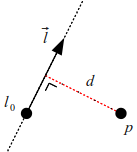
\includegraphics[width=2.5cm]{distlp.png}
\end{minipage}
\end{tabular}

\begin{tabular}{l l}
\begin{minipage}{0.7\textwidth}
\begin{description}
\item[linePointClosestToPoint] This method is used to determine the
  point on a line that is closest to a given point. The line, dashed
  black in the example to the right, is defined by a point vector
  $l_0$ and a direction vector $\vec{l}$, the point $p_0$ is also a
  point vector. The method returns the coordinates of point $p_1$.
\end{description}
\end{minipage}
&
\begin{minipage}{0.3\textwidth}
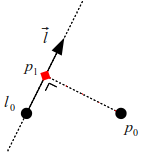
\includegraphics[width=2.5cm]{pointlcp.png}
\end{minipage}
\end{tabular}

\begin{tabular}{l l}
\begin{minipage}{0.7\textwidth}
\begin{description}
\item[intersectVectorPlane] Determine the coordinates of the
  intersection of a line with a plane. The line, dashed black in the
  example to the right, is defined by a point vector $l_0$ and a
  direction vector $\vec{l}$. The plane is defined by the vector $(a,
  b, c, d)^T$, such that $ax + by + cz = d$. In this representation,
  the vector $(a,b,c)^T$ is normal to the plane and $d$ is the
  distance of the plane to the origin of the reference frame. The
  method returns the coordinates of point $p$.
\end{description}
\end{minipage}
&
\begin{minipage}{0.3\textwidth}
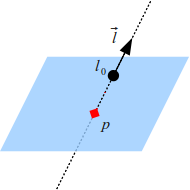
\includegraphics[width=3cm]{intersectvectorplane.png}
\end{minipage}
\end{tabular}

\section{Types}

The {\tt Types} class holds many useful types and enumerations, used
throughout the library. Here is a brief overview of these, but also
make sure to look at the code documentation.
\begin{description}
\item[PlayMode] This enumeration list all the possible play modes. For
  modes of which there are two side variants, e.g. kick-off and free
  kick, there is also an 'us' and a 'them' version. It is recommended
  to use these instead of the left/right versions, and all {\tt
    libbats} modules use the us/them versions. For instance, if the
  left team gets the kick-off, and our team plays on the right, {\tt
    WorldModel::getPlayMode()} will return {\tt Types::KICKOFF\_THEM}.
\item[Side] A simple enumeration to discern left and right in a
  human-readable manner.
\item[Joint] An enumeration of all the agent's joints. This is for
  instance used to get the current angle of a joint from the {\tt
    AgentModel}:
\begin{lstlisting}[frame=single]
  // Get angle of the first joint of the left arm, in radians double
  angle = am.getJoint(Types::LARM1)->angle.getMu()(0);
\end{lstlisting}
\item[BodyPart] An enumeration of all the agent's body parts. This is
  for instance used to get the current location of a body part from
  the {\tt AgentModel}:
\begin{lstlisting}[frame=single]
// Get the position of the left foot, relative to the torso
Vector3d pos = am.getBodyPart(Types::LFOOT)->transform.translation;
\end{lstlisting}
\item[Object] This enumeration lists all objects in the environment,
  such as the ball, players, opponents, and landmarks. For the latter
  there are left/right and us/them versions. Again, it is recommended
  to use the us/them variants:
\begin{lstlisting}[frame=single]
// Get the location of the first post of the opponent goal,
// in local coordinates
Vector3d pos = localizer.getLocaltionLocal(Types::GOAL1THEM)->getMu();
\end{lstlisting}
\end{description}

